\documentclass[titlepage,a4paper,11pt]{article}
\usepackage[pdfborder={0 0 0}]{hyperref}
\usepackage{fontspec}
\usepackage[hmargin=2.54cm,vmargin=1.91cm]{geometry}
\usepackage{parskip}
\usepackage{wrapfig}
\usepackage{multirow}
\usepackage[english]{babel}
\usepackage{longtable}
\usepackage{float}
\usepackage{graphicx}
\usepackage[table]{xcolor}
\usepackage{biblatex}

%	-- Some important declarations --
%	-- Bibliography
\bibliography{myrefs}

%	-- Tableshade color
\definecolor{tableShade}{HTML}{F1F5FA}

%	-- Project info
\def \project {Defense of the Guardian Gnome}
\def \objective {guardian gnome}

%	-- Font Style (uses Xelatex engine (Unicode))
\setromanfont{Century Gothic}

%	-- Date of last run (frontpage)
\date{\today}

\begin{document}

%	-- Title Page	
\title{Requirement Specification\\
 		TDT4240 - XNA Game Project}

\author{Dag Øyvind Tornes\\
 		Sibte-Haider Syed\\ 
		Robin Kåveland Hansen\\}
\maketitle

\pagestyle{empty}
\tableofcontents
\clearpage
\pagestyle{plain}
\pagenumbering{arabic}

%	-- Actual report
\section{Introduction}
	\subsection{About this document}
		This document describes the requirements that have been developed for \project,
a game developed for the XNA platform. It describes the functional requirements
and thus a high-level overview of how the game should play. There are also some
scenarios for content development that describe the quality requirements imposed
on the system. Chapter \ref{concepts} describes the concept behind the game on
a high level, as well as some discussion around some game design choices that
have been made at this time or will have to be made in the future. Chapter
\ref{funcreq} lays down the functional requirements that were decided on.
Chapter \ref{qualreq} deals with the quality requirements in detail, as well as
some scenarios that might be relevant for \project. Chapter \ref{constraints}
describes in some detail the constraints that were imposed on the game by either
the developers, or the technology used.


\subsection{Concepts and ideas}
	\label{concepts}
	The idea behind the game is to defend an object of great value, the \objective.
This object is contineously assailed by enemies, from here on out known as \emph{creeps}.
Creeps are fortunately not very intelligent, and so move in certain predetermined
paths toward the \objective, allowing players to intercept them and defeat them.
Once the \objective is destroyed, or the last creep defeated, the game ends.

Each player controls a \emph{hero} that defends against the creeps. Heroes gain
\emph{experience} upon defeating creeps, and eventually gain levels, and new abilities.
As heroes grow more powerful, so too do creeps.


\section{Functional Requirements}
	\label{funcreq}
	%	Functional Requirements 
%	TableShading is on
%	Template style

\begin{table}[H]
	\resizebox{\textwidth}{!}{
	\rowcolors{0}{white}{tableShade}
	\begin{tabular}{p{5cm} | p{12cm}}
    	\hline
		\textbf{ID:} 			& 	\textbf{FR1} 												 \\ 
		\hline
    	
		\textbf{Priority:}		&	High														 \\
		\textbf{Description}	& 	The game will run on Xbox 360								 \\ 
		\textbf{Rationale}		& 	Please see chapter \ref{constraints}						 \\
		\hline
    \end{tabular}
	\label{tab:functional1}}
\end{table}


\begin{table}[H]
	\resizebox{\textwidth}{!}{
	\rowcolors{0}{white}{tableShade}
	\begin{tabular}{p{5cm} | p{12cm}}
    	\hline
		\textbf{ID:} 			& 	\textbf{FR2} 												\\ 
		\hline
    	
		\textbf{Priority:}		&	High														\\
		\textbf{Description}	& 	The game is multiplayer. It shall support minimum two  
									players, and maximum 4 players								\\ 
		\textbf{Rationale}		& 	The project assignment states that the game must be 
		 							multiplayer. The Xbox 360 natively supports 4 controllers
									wirelessly. The console supports a maximum of 7 controllers,
									where three controllers are wired. We have landed on the 
									conclusion to support 4, so all can play wirelessly \\
		\hline
    \end{tabular}
	\label{tab:functional2}}
\end{table}

\begin{table}[H]
	\resizebox{\textwidth}{!}{
	\rowcolors{0}{white}{tableShade}
	\begin{tabular}{p{5cm} | p{12cm}}
    	\hline
		\textbf{ID:} 			& 	\textbf{FR3} 												\\ 
		\hline
    	
		\textbf{Priority:}		&	High														\\
		\textbf{Description}	& 	The game must support pausing and unpausing.				\\ 
		\textbf{Rationale}		& 	In order to meet the conceptual model of a gamer,
		 							we must have this feature\\
		\hline
    \end{tabular}
	\label{tab:functional3}}
\end{table}

\begin{table}[H]
	\resizebox{\textwidth}{!}{
	\rowcolors{0}{white}{tableShade}
	\begin{tabular}{p{5cm} | p{12cm}}
    	\hline
		\textbf{ID:} 			& 	\textbf{FR4} 												\\ 
		\hline
    	
		\textbf{Priority:}		&	High														\\
		\textbf{Description}	& 	The game is in 2D											\\ 
		\textbf{Rationale}		& 	To ensure focus on architecture								\\
		\hline
    \end{tabular}
	\label{tab:functional4}}
\end{table}

\begin{table}[H]
	\resizebox{\textwidth}{!}{
	\rowcolors{0}{white}{tableShade}
	\begin{tabular}{p{5cm} | p{12cm}}
    	\hline
		\textbf{ID:} 			& 	\textbf{FR5} 												\\ 
		\hline
    	
		\textbf{Priority:}		&	High														\\
		\textbf{Description}	& 	The game must be able to \emph{spawn} creeps				\\ 
		\textbf{Rationale}		& 	To provide a challenge / objective for the player			\\
		\hline
    \end{tabular}
	\label{tab:functional5}}
\end{table}

\begin{table}[H]
	\resizebox{\textwidth}{!}{
	\rowcolors{0}{white}{tableShade}
	\begin{tabular}{p{5cm} | p{12cm}}
    	\hline
		\textbf{ID:} 			& 	\textbf{FR6} 												\\ 
		\hline
    	
		\textbf{Priority:}		&	High														\\
		\textbf{Description}	& 	Each player controls a \emph{hero}							\\ 
		\textbf{Rationale}		& 	To provide challenge for the player							\\
		\hline
    \end{tabular}
	\label{tab:functional6}}
\end{table}

\begin{table}[H]
	\resizebox{\textwidth}{!}{
	\rowcolors{0}{white}{tableShade}
	\begin{tabular}{p{5cm} | p{12cm}}
    	\hline
		\textbf{ID:} 			& 	\textbf{FR7} 												\\ 
		\hline
    	
		\textbf{Priority:}		&	High														\\
		\textbf{Description}	& 	Creeps attack either a hero or the structure to be defended	\\ 
		\textbf{Rationale}		& 	To provide challenge for the player							\\
		\hline
    \end{tabular}
	\label{tab:functional7}}
\end{table}

\begin{table}[H]
	\resizebox{\textwidth}{!}{
	\rowcolors{0}{white}{tableShade}
	\begin{tabular}{p{5cm} | p{12cm}}
    	\hline
		\textbf{ID:} 			& 	\textbf{FR8} 												\\ 
		\hline
    	
		\textbf{Priority:}		&	Medium														\\
		\textbf{Description}	& 	A player cannot attack another player						\\ 
		\textbf{Rationale}		& 	The game is cooperative										\\
		\hline
    \end{tabular}
	\label{tab:functional8}}
\end{table}

\begin{table}[H]
	\resizebox{\textwidth}{!}{
	\rowcolors{0}{white}{tableShade}
	\begin{tabular}{p{5cm} | p{12cm}}
    	\hline
		\textbf{ID:} 			& 	\textbf{FR9} 												\\ 
		\hline
    	
		\textbf{Priority:}		&	High														\\
		\textbf{Description}	& 	A hero / player has a limited amount of health	and resource\\ 
		\textbf{Rationale}		& 	The game is cooperative, and adding depth to the game		\\
		\hline
    \end{tabular}
	\label{tab:functional9}}
\end{table}

\begin{table}[H]
	\resizebox{\textwidth}{!}{
	\rowcolors{0}{white}{tableShade}
	\begin{tabular}{p{5cm} | p{12cm}}
    	\hline
		\textbf{ID:} 			& 	\textbf{FR10} 												\\ 
		\hline
    	
		\textbf{Priority:}		&	High														\\
		\textbf{Description}	& 	A hero gains experience/resources/bonuses					\\ 
		\textbf{Rationale}		& 	To make the game more challenging and adding depth			\\
		\hline
    \end{tabular}
	\label{tab:functional10}}
\end{table}


\begin{table}[H]
	\resizebox{\textwidth}{!}{
	\rowcolors{0}{white}{tableShade}
	\begin{tabular}{p{5cm} | p{12cm}}
    	\hline
		\textbf{ID:} 			& 	\textbf{FR11} 												\\ 
		\hline
    	
		\textbf{Priority:}		&	High														\\
		\textbf{Description}	& 	A hero / player have a limited amount of health	 / lives	\\ 
		\textbf{Rationale}		& 	The game must be challenging								\\
		\hline
    \end{tabular}
	\label{tab:functional11}}
\end{table}

\begin{table}[H]
	\resizebox{\textwidth}{!}{
	\rowcolors{0}{white}{tableShade}
	\begin{tabular}{p{5cm} | p{12cm}}
    	\hline
		\textbf{ID:} 			& 	\textbf{FR12} 												\\ 
		\hline
    	
		\textbf{Priority:}		&	Medium														\\
		\textbf{Description}	& 	If a hero dies, the player must wait a fixed amount of time
									before respawning. Should increase as the player advances 	\\ 
		\textbf{Rationale}		& 	The game must be challenging								\\
		\hline
    \end{tabular}
	\label{tab:functional12}}
\end{table}

\begin{table}[H]
	\resizebox{\textwidth}{!}{
	\rowcolors{0}{white}{tableShade}
	\begin{tabular}{p{5cm} | p{12cm}}
    	\hline
		\textbf{ID:} 			& 	\textbf{FR13} 												\\ 
		\hline  	
		\textbf{Priority:}		&	Medium														\\
		\textbf{Description}	& 	A hero has special 2 abilities (fixed amount)				\\ 
		\textbf{Rationale}		& 	The game must be challenging								\\
		\hline
    \end{tabular}
	\label{tab:functional13}}
\end{table}


\begin{table}[H]
	\resizebox{\textwidth}{!}{
	\rowcolors{0}{white}{tableShade}
	\begin{tabular}{p{5cm} | p{12cm}}
    	\hline
		\textbf{ID:} 			& 	\textbf{FR14} 												\\ 
		\hline
    	
		\textbf{Priority:}		&	Medium														\\
		\textbf{Description}	& 	A hero has skills: Attack speed, health, strength, agility, 
									movement speed and intelligence								\\ 
		\textbf{Rationale}		& 	The game must be challenging								\\
		\hline
    \end{tabular}
	\label{tab:functional14}}
\end{table}

\begin{table}[H]
	\resizebox{\textwidth}{!}{
	\rowcolors{0}{white}{tableShade}
	\begin{tabular}{p{5cm} | p{12cm}}
    	\hline
		\textbf{ID:} 			& 	\textbf{FR15} 												\\ 
		\hline
    	
		\textbf{Priority:}		&	Low															\\
		\textbf{Description}	& 	A hero can buy items to enhance abilities or skills			\\ 
		\textbf{Rationale}		& 	The game is cooperative										\\
		\hline
    \end{tabular}
	\label{tab:functional15}}
\end{table}

\begin{table}[H]
	\resizebox{\textwidth}{!}{
	\rowcolors{0}{white}{tableShade}
	\begin{tabular}{p{5cm} | p{12cm}}
    	\hline
		\textbf{ID:} 			& 	\textbf{FR16} 												\\ 
		\hline
    	
		\textbf{Priority:}		&	High															\\
		\textbf{Description}	& 	A new player cannot join the game once it has started			\\ 
		\textbf{Rationale}		& 	The game is cooperative										\\
		\hline
    \end{tabular}
	\label{tab:functional16}}
\end{table}

\begin{table}[H]
	\resizebox{\textwidth}{!}{
	\rowcolors{0}{white}{tableShade}
	\begin{tabular}{p{5cm} | p{12cm}}
    	\hline
		\textbf{ID:} 			& 	\textbf{FR17} 													\\ 
		\hline
    	
		\textbf{Priority:}		&	Medium															\\
		\textbf{Description}	& 	Passive abilities does not need to be activated by the player	\\ 
		\textbf{Rationale}		& 	According to the conceptual model of this genre of games		\\
		\hline
    \end{tabular}
	\label{tab:functional17}}
\end{table}

\begin{table}[H]
	\resizebox{\textwidth}{!}{
	\rowcolors{0}{white}{tableShade}
	\begin{tabular}{p{5cm} | p{12cm}}
    	\hline
		\textbf{ID:} 			& 	\textbf{FR18} 													\\ 
		\hline
    	
		\textbf{Priority:}		&	Medium															\\
		\textbf{Description}	& 	Active abilities needs to be activated by the player and has a 
		 							\emph{cooldown} once used \\ 
		\textbf{Rationale}		& 	According to the conceptual model of this genre of games		\\
		\hline
    \end{tabular}
	\label{tab:functional18}}
\end{table}

\begin{table}[H]
	\resizebox{\textwidth}{!}{
	\rowcolors{0}{white}{tableShade}
	\begin{tabular}{p{5cm} | p{12cm}}
    	\hline
		\textbf{ID:} 			& 	\textbf{FR19} 													\\ 
		\hline
    	
		\textbf{Priority:}		&	High															\\
		\textbf{Description}	& 	The game ends if the \emph{Guardian Gnome} survives all the \emph{waves},
		  							or the \emph{Guardian Gnome} is killed by the creeps \\ 
		\textbf{Rationale}		& 	To give the player an winning scenario, and a failure scenario	\\
		\hline
    \end{tabular}
	\label{tab:functional19}}
\end{table}

\begin{table}[H]
	\resizebox{\textwidth}{!}{
	\rowcolors{0}{white}{tableShade}
	\begin{tabular}{p{5cm} | p{12cm}}
    	\hline
		\textbf{ID:} 			& 	\textbf{FR20} 													\\ 
		\hline
    	
		\textbf{Priority:}		&	High															\\
		\textbf{Description}	& 	Each player will have his score shown while playing: kills + points \\ 
		\textbf{Rationale}		& 	To introduce a competitive scenario even though it is cooperative	\\
		\hline
    \end{tabular}
	\label{tab:functional20}}
\end{table}


\section{Quality Requirements}
	\label{qualreq}
	The primary quality attribute for this project is modifiability, while the
secondary one is usability. It is important to the group that it should not
take very long for a gamer to get to grips with the game, so as to push focus
away from learning it and onto mastering it.

\subsection{Quality Requirement Listing: Modifiability}

\begin{table}[H]
  \resizebox{\textwidth}{!}{
    \rowcolors{0}{white}{tableShade}
    \begin{tabular}{p{5cm} | p{12cm}}
      \hline
      \textbf{ID} & \textbf{QR1}  \\
      \hline
      \textbf{Source} &  Developer \\
      \textbf{Stimulus} &  Developer wants to add hero \\
      \textbf{Environment} &  Design time \\
      \textbf{Artifact} & Code \\
      \textbf{Response} & Adds code for hero \\
      \textbf{Response Measure} & Code modification takes place only in trigger and ability code\\
      \hline
    \end{tabular}
    \label{tab:quality1}}
\end{table}

\begin{table}[H]
  \resizebox{\textwidth}{!}{
    \rowcolors{0}{white}{tableShade}
    \begin{tabular}{p{5cm} | p{12cm}}
      \hline
      \textbf{ID} & \textbf{QR2}  \\
      \hline
      \textbf{Source} &  Developer \\
      \textbf{Stimulus} &  Developer wants to add new game-mode\\
      \textbf{Environment} &  Design time \\
      \textbf{Artifact} & Code \\
      \textbf{Response} & Adds code for new game-mode \\
      \textbf{Response Measure} & No code modification required except in menu
      system\\
      \hline
    \end{tabular}
    \label{tab:quality2}}
\end{table}

\begin{table}[H]
  \resizebox{\textwidth}{!}{
    \rowcolors{0}{white}{tableShade}
    \begin{tabular}{p{5cm} | p{12cm}}
      \hline
      \textbf{ID} & \textbf{QR3}  \\
      \hline
      \textbf{Source} &  Graphical Designer \\
      \textbf{Stimulus} &  Designer wants to change hero sprite \\
      \textbf{Environment} &  After compile time \\
      \textbf{Artifact} & Hero data \\
      \textbf{Response} & Old sprite replaced with new sprite \\
      \textbf{Response Measure} & Takes no more than 2 minutes and no
      code modification or recompilation required \\
      \hline
    \end{tabular}
    \label{tab:quality3}}
\end{table}

\begin{table}[H]
  \resizebox{\textwidth}{!}{
    \rowcolors{0}{white}{tableShade}
    \begin{tabular}{p{5cm} | p{12cm}}
      \hline
      \textbf{ID} & \textbf{QR4}  \\
      \hline
      \textbf{Source} &  Game Designer\\
      \textbf{Stimulus} &  Game Designer wants to adjust unbalanced hero\\
      \textbf{Environment} &  After compile time \\
      \textbf{Artifact} & Hero data \\
      \textbf{Response} & Hero damage and other stats adjusted \\
      \textbf{Response Measure} & Game ready to test new hero stats without
      requiring code modification or recompilation \\
      \hline
    \end{tabular}
    \label{tab:quality4}}
\end{table}

\subsection{Quality Requirement Listing: Usability}

\begin{table}[H]
  \resizebox{\textwidth}{!}{
    \rowcolors{0}{white}{tableShade}
    \begin{tabular}{p{5cm} | p{12cm}}
      \hline
      \textbf{ID} & \textbf{QR5}  \\
      \hline
      \textbf{Source} &  Player \\
      \textbf{Stimulus} &  Player wants to learn the game controls\\
      \textbf{Environment} &  Runtime \\
      \textbf{Artifact} & Game \\
      \textbf{Response} & Game starts and player plays \\
      \textbf{Response Measure} & It takes no longer than 3 minutes before
      the player is able to control and attack with the hero \\
      \hline
    \end{tabular}
    \label{tab:quality5}}
\end{table}

\begin{table}[H]
  \resizebox{\textwidth}{!}{
    \rowcolors{0}{white}{tableShade}
    \begin{tabular}{p{5cm} | p{12cm}}
      \hline
      \textbf{ID} & \textbf{QR6}  \\
      \hline
      \textbf{Source} &  Players \\
      \textbf{Stimulus} &  2 or more players want to play multiplayer \\
      \textbf{Environment} &  Runtime \\
      \textbf{Artifact} & Menusystem \\
      \textbf{Response} & Game starts multiplayer mode \\
      \textbf{Response Measure} & It takes less than 5 keypresses per
      player to get started. \\
      \hline
    \end{tabular}
    \label{tab:quality6}}
\end{table}


\section{COTS Components}
	\label{components}
	XNA is a Microsoft developed set of tools for developing games. It is available
primarily for the Microsoft Windows, Windows Mobile and Xbox 360 platforms, though
it has been ported to the cross-platform Mono framework\footnote{This work is not
  complete}. It allows easy creation of both 3-dimensional and 2-dimensional games,
and supports audio and multiple input devices. It also supports many common data
formats for both visual and audio. Typically, one develops games for XNA with the
usage of one of the (So far) 5 revisions of XNA Game Studio.


\section{Constraints}
	\label{constraints}
	\subsection{Technological constraints}
Newer XNA versions are only widely supported on the Windows and Xbox 360
platforms, and as such these were our only available target platforms. We decided
to narrow this down further to only the Xbox 360 platform due to the difficulty
of adopting the concept to hot-seat multiplayer mode, and the time constraints
of the course making it difficult to implement multiplayer over network. This
in turn means that player control happens with the Xbox 360 controller, which
constrains our input to something that makes sense with this. Due to the usage
of XNA, we are also forced to use a Microsoft license if we want the game to be
published.
\begin{figure}
  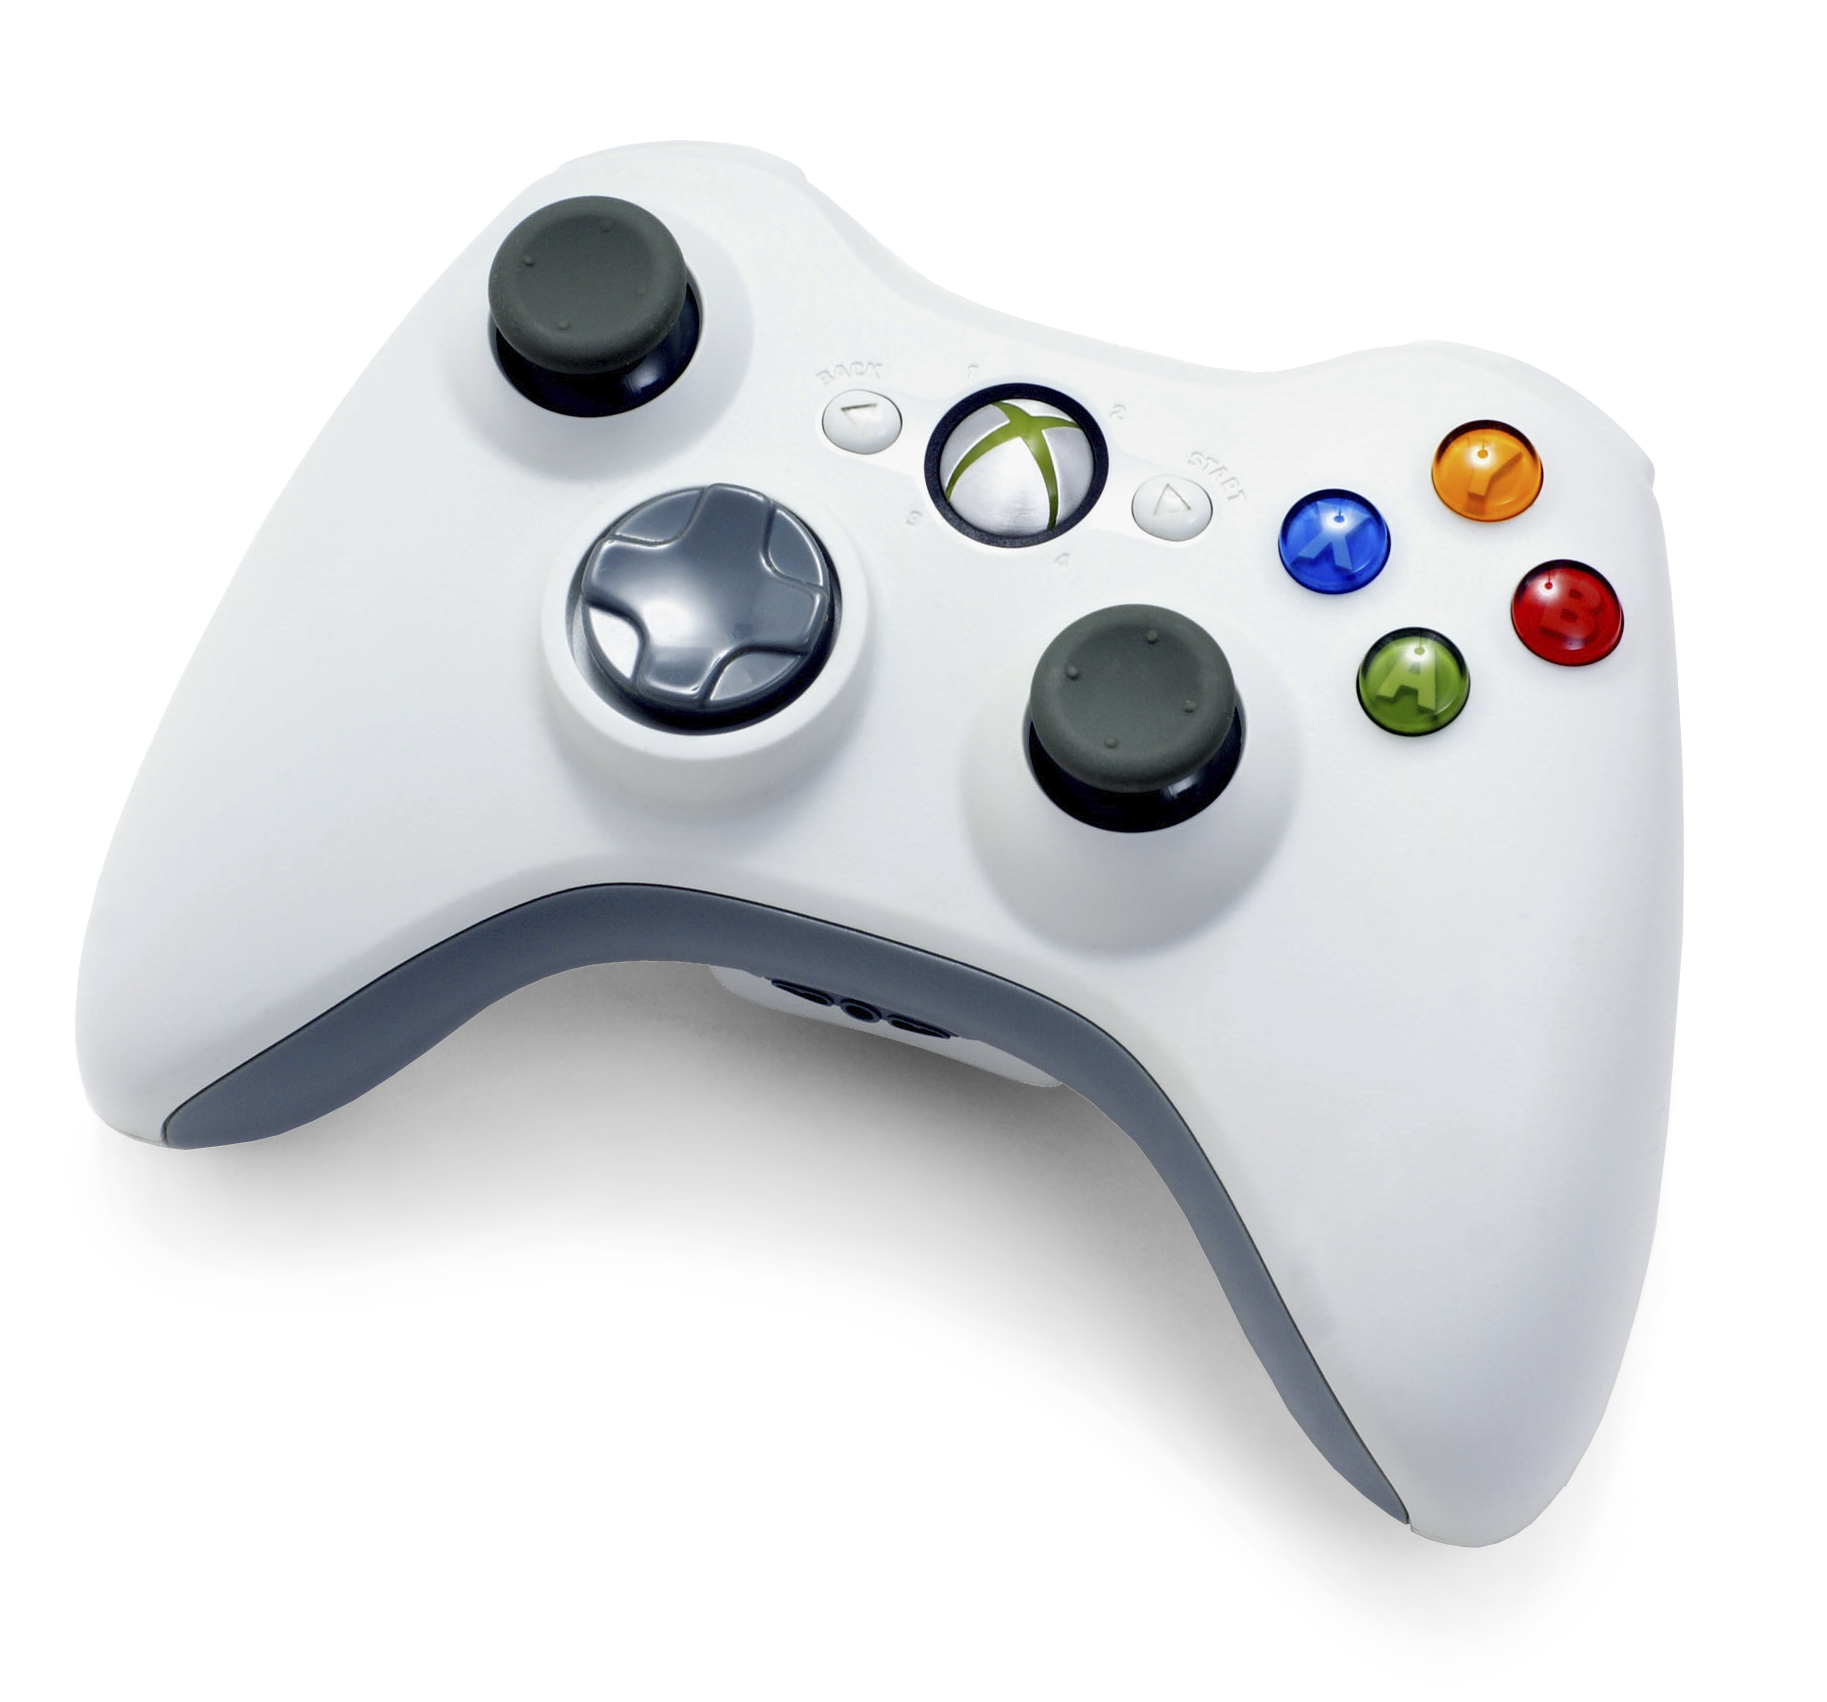
\includegraphics[scale=0.2]{graphics/controller}
  \caption{The Xbox 360 controller, showing the available inputs}
\end{figure}

\subsection{Self-imposed constraints}
We decided to limit ourselves to 2-dimensional graphics, letting us focus more
on architecture and game engine creation than 3-dimensional content creation,
which is a time-consuming process. Additionally, we know from experience that
designing intelligent game AI is relatively time-consuming and challenging.
It is however possible to make captivating games that do not have much in the way
of artificial intelligence in the opponents, so we felt it safe to not prioritize
this. 


\section{Issues}
	\label{issues}
	No issues yet

\printbibliography


\section{Revision history}

\begin{table}[H]
  \begin{tabular}{| c | c | p{5cm} |}
    \hline
    0.1 & 25.02.2011 & Initial revision of this document. \\
	0.2 & 13.03.2011 & FR10 was split into to requirements (now FR10 and FR 11). Easier to address and test. \\
	0.3 & 05.04.2011 & Updated the ID format from QR to-> M for modifiability, U for Usability according to feedback from staff\\
    \hline
  \end{tabular}
\end{table}

\end{document}
	\bibliographystyle{plainnat}